\chapter{Grundlagen}

\section{Datenquellen}
Die Datengrundlage für dieses Projekt sind Daten des Mars Orbiter Laser Altimeter (MOLA), einem Höhenmessgerät an Bord des 
               

% Beschreibe die MOLA Mission und mit welchen Instrumenten sie erfasst wurden
% erwähne Digital Elevation Models (DEMs) und das sie ein rasterformat sind, also immer gleiche Abstände zwischen Datenpixeln die unabhängig von der Tpographie des Marses erstellt wurden

% Beschreibe die Parameter (Auflösung, Datengröße, Genauigkeit (horizontal/vertikal))
% Beschreibe das Datenformat und Unterschiede / Vor- und Nachteile

%% https://pds-geosciences.wustl.edu/missions/mgs/megdr.html vs. https://astrogeology.usgs.gov/search/details/Mars/GlobalSurveyor/MOLA/Mars_MGS_MOLA_DEM_mosaic_global_463m
%% entscheide dich für die 2., auch wenn du das Format des 1. besser findest <-- da beim 1. Daten fehlen und das Mapping Auf Kugel dann schwierig wird
%% beschreibe, warum das Format nicht gut ist -> beschreibe Aufbau von TIFF Dateien (Container-Format, Daten an verschiedenen Stellen in der Datei) -> decoder benötigt

\section{OpenGL}
% nur für dieses Projekt relevante Aspekte von OpenGL
% Grundlagen: nur Interface, verschiedene Implementationen in Form von Driver
% existiert auch WebGL ← Unterschiede und Gemeinsamkeiten, z.B. 
% Erklärung Shader Pipeline
% Shadersprache GLSL
% Erklärung Kommunikation mit Shader (Attribut vs Uniform)
% Koodinaten Systeme -> wie verlaufen die Achsen (positive x-Achse nach rechts, positive y-Achse nach oben und positive z-Achse in den Bildschirm hinein)

\section{Datenreduzierung}

\subsection{Datenmenge}\label{datenmenge}
Der beschriebene MOLA-Datensatz besitzt eine Breite von 46080 Pixeln und eine Höhe von 23040 Pixeln. Jeder Pixel ist dabei 16 bit groß, sodass die Rohdaten an sich eine Größe von 1,98 GB besitzen\cite{molaDataExtended}. Um daraus ein 3D-Modell zu erstellen, müssen neben den Höhenwerten natürlich auch die x- und z-Position erfasst werden, welche sich aus dem Rasterformat der Daten errechnen lassen. Erschwerend hinzu kommt, dass der kleinste numerische Datentyp in GLSL 32 bit groß ist\cite[Abschnitt 4.1, S. 23]{glslSpec} und sich die Höhendaten so nicht effizient speichern lassen. Eine entsprechende Erweiterung (\textit{extension}) von GLSL um 16 bit Typen mit dem Namen EXT\_shader\_16bit\_storage existiert, befindet sich allerdings erst in der Entwurfsphase und kann daher nicht genutzt werden. Die reinen Vertex-Daten besitzen also eine Größe von 11,88 GB. Weitere Daten pro Vertex (zum Beispiel Normalenvektoren) werden für dieses Projekt nicht benötigt. Allerdings können diese Vertex-Daten in dieser Form nicht an OpenGL übergeben werden, da erst Polygone (OpenGL Primitives) daraus erstellt werden müssen. Im einfachsten Fall sind dies für ein Rastermodell natürlich Vierecke (GL\_QUAD), diese Form ist allerdings veraltet und sollten nicht mehr benutzt werden. Stattdessen müssen die Vertex-Daten  Dreiecke (GL\_TRIANGLE) beschreiben. Da in einem Rastermodell aus Dreiecken natürlich ein Vertex 6 mal wiederholt werden müsste, gibt es eine effizientere Beschreibung der Polygone: Indexierung. Dabei wird ein Array an OpenGL übergeben, welche die Reihenfolge der Vertices als deren Position im ursprünglichen Vertex-Array kodiert (siehe Abbildung \ref{indexing}). 

\begin{figure}[H]
  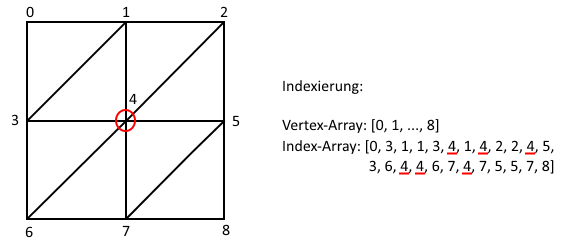
\includegraphics{indexing.png}
  \caption{Indexierung eines Raster-Modells}
  \label{indexing}
\end{figure}

Durch diese Technik wird das Wiederholen eines Vertex verhindert, allerdings ist auch hier ein Speicherverbrauch zu berechnen. Der Index entspricht dabei einer Größe von 32 bit und die Anzahl lässt sich mit folgender Formel berechnen: $Anzahl = 6 * (H\ddot{o}he - 1) * (Breite - 1) = 6.369.684.486$. Dadurch werden weitere 23,73 GB benötigt, wodurch der Gesamtspeicherverbrauch auf 35,61 GB steigt. Da dies, auch ohne nicht-funktionale Anforderungen definiert zu haben, nicht in einen durchschnittlichen Grafikspeicher passt, sind Maßnahmen zur Reduzierung der Daten zwingend erforderlich.

\subsection{Verlustfrei}
Das Durchführen von verlustfreien Methoden zur Reduzierung der Datenmenge ist natürlich immer den verlustbehafteten Methoden vorzuziehen, da ...
Die einfachste Möglichkeit, ist die Entfernung von Redundanzen. Diese können auf Grund des Rasterformats der Daten vorhanden sein, da die Abstände zwischen den Datenpixeln laut Definition einem festen Wert entsprechen müssen. Die hohe horizontale Datenauflösung von 463m bei einer natürlichen Topographie führt zu der statistischen Annahme, dass dabei Redundanzen auftreten. Hier stellt sich die Frage, was eigentlich eine Redundanz im Kontext von 2D Höhenwerten ist. Ein Auffinden von gleichen Werten in einem 3x3 Raster ist der einfachste Fall. Wichtig hierbei ist, dass nicht etwa ein einfaches Wiederholen von Werten bereits eine Redundanz ist, da auch das Darstellen einer flachen Ebene eine wichtige Information ist. Allerdings können Redundanzen auch bei einer geneigten Ebene auftreten, bei der sich benachbarte Höhenwerte unterscheiden. Der generelle Fall zur Beschreibung ist das Vorhandensein einer linearen Abhängigkeit zwischen Werten in \textbf{allen} Spalten und Reihen eines mindestens 3x3 großen Rasters\cite{topoDataReduction}. Wichtig hierbei ist, dass immer der 2D Kontext beachtet werden muss. Es können sich beliebig viele Werte in einer Reihe oder Spalte wiederholen, ohne das dies eine Redundanz darstellt, wenn auch nur eine Spalte oder Reihe im Raster diese lineare Abhängigkeit nicht aufweist. Um das Vorhandensein von Redundanzen im MOLA Datensatz zu beweisen, wurde ein Script erstellt (siehe \ref{redundanzberechnung}). Dies zeigt, dass insgesamt 65.866.353 Datenpixel redundant sind, was einem Prozentsatz von 6,20\% entspricht. Dabei existieren 10.395.105 redundante Teilraster, das größte von ihnen besitzt immerhin eine Fläche von 278,68km².

Eine andere Möglichkeit eine verlustfreie Reduktion zu erreichen, ist die Daten zu entfernen, die vom Benutzer nicht gesehen werden können. Das betrifft explizit nicht den Punkt, dass Unterschiede auf Grund der Physiologie des menschlichen Auges nicht wahrgenommen werden können, da dies trotzdem einem theoretischen Informationsverlust entspricht.



\subsection{Verlustbehaftet}
Das Durchführen von verlustfreien Methoden allein reicht nicht aus, um den Speicherverbrauch auf ein akzeptables Niveau zu senken.

% systematische reduktion, mit fester Schritteite (stride) über die Daten iterieren -> Vorteil: die Indexierung bleibt erhalten nur die Abstände vergößern sich
% geringe Änderungen in einem 3D Kontekt, auch oft als geringe räumliche Frequenz beschrieben, 

\subsection{Probleme}
Ein zentrales Problem bei der Entfernung von Redundanzen ist die Indexierung des Modells. In einem reinen Raster-Modell lassen sich die Indices trivial berechnen, da sie immer einem gleichmäßigem Muster folgen. Jetzt existieren natürlich Lücken in den Vertex-Daten und eine neues Polygon Netz muss gefunden werden. 

Auch besteht das Problem, diese Lücken in einem Datenformat darzustellen. Normalerweise besteht immer der gleiche Abstand zwischen zwei benachbarten Datenpunkte, wenn jetzt einfach Vertices entfernt werden, dann ändern sich die Abstände und dies muss irgendwie kodiert werden.




Wie beschrieben, ist die Unterteilung des Gesamtmodells in Abschnitte ein zentraler Aspekt der Anwendung um das frustum- und occlusion culling durchführen zu können. Die führt aber zu einer Einschränkung bei der Entfernung von Redundanzen, die über Abschnittsgrenzen hinaus gehen würden. Diese stellen plötzlich keine Redundanz mehr da, da die Kanten des Abschnitts natürlich definiert werden müssen. Auch sollen per Design Abschnitte keinen Zugriff auf Vertex-Daten anderer Abschnitte erhalten (schon allein um Daten nicht unnötig im RAM zu halten). Dies führt dazu, dass das Entfernen von Redundanzen zur Laufzeit geschehen muss, da




Einzelne Abschnitte haben keinerlei Zugriff auf Daten der anderen Abschnitte und benötigen eine 



% Abschnitt, der erstmal die vollständige Datengröße beschreibt
% außerdem ist es ein Rasterformat, also feste Abstände zwischen einzelnen Datenpunkten

% verlustfrei: alles was nicht im Sichtbereich der Kamera liegt (Frustum Culling) und alles, was durch andere Dinge verdeckt wird (Occlusion Culling) -> andere Seite des Globus
% dazu Unterteilung der Welt in Abschnitte (chunks) und nur Anzeigen der Abschnitte, welche den Sichtbreich auch nur ansatzweise schneiden und nicht vollständig durch andere Abschnitte verdeckt sind
% verlustbehaftet: 
% hier ausnutzen, dass zum Beispiel bei geringen Zoomstufen Unterschiede in den Daten nicht mehr wahrgenommen werden können
% Außerdem: Entfernung von Redundanzen -> da Rasterformat , hier ist es abhängig von der Komplexität des Terrains,

% Redukttion der Datenmenge in festgelegten Schritten (stride), systemetaische Reduktion
% Reduktion der Datenmenge abhängig vom umliegenden Terrain -> ähnliche vertices müssen nicht wiederholt werden,
% gerade bei natürlichen Daten gibt es sehr ähnliche Pubkt

% eine Plane besteht zwar auf 4 Eckpunkten, allerdings muss sie in OpenGL Primitives zerlegt werden -> dies sind normalerweise Dreiecke
% es existieren auch Quad-Primitives, diese sind jedoch veraltet und sollten nicht mehr benutzt werden

% also 6 Eckpunkte, da ja jeder Eckpunk auch Teil des benachbartenn PLane ist, wird insgesamt ein Eckpunkt 6 mal wiederholt (siehe kleine Grafik) -> also wird bei der Erzeugung des Modell eine Indexierung vorgenommen, einfach eine Liste mit Indexen die eine die Liste mit den Vertex-Daten referenziert ->

% bei der systematischen Reduktion ist das kein Problem, die Indixierung des Raster Modells bleibt erhalten, nur die Abstände zwischen den Vertices erhöhen sich

% erwähne die Formel um aus einem 1D Array ein 2D Array zu erstellen

% bei der asymetrischen Reduktion kann nicht mehr aus dem 1D Vertex-Format auf eine Indexierung geschlossen werden, also muss hier ein 2D Format gesendet werden was die entfernen
% Vertex-Daten kennzeichnet